\documentclass[12pt,a4paper]{article}
\usepackage[UTF8]{ctex}
\usepackage{amsmath}
\usepackage{geometry}
\usepackage{graphicx}
\usepackage{subcaption}
\geometry{margin=2.2cm}

\title{量子信息基础第六次作业第二题报告}
\author{}
\date{}

\begin{document}
\maketitle

\section*{计算方法}
本文使用有限差分方法将一维定态薛定谔方程离散化，构造哈密顿矩阵并求解本征值与本征函数。程序使用 \texttt{Python} 编写，网格点数取 $N=800$。

\section*{(a) 50 nm 无限深势阱的势能曲线和波函数}
对于宽度为 $50\,\mathrm{nm}$ 的无限深势阱，数值得到前四个能级为
\[
E_1=0.1502\ \mathrm{meV},\quad
E_2=0.6008\ \mathrm{meV},\quad
E_3=1.3518\ \mathrm{meV},\quad
E_4=2.4031\ \mathrm{meV}.
\]
从图中可以看到，基态波函数无节点，第一到第三激发态的节点数依次增加，符合一维束缚态波函数的基本规律。

\begin{figure}[h]
    \centering
    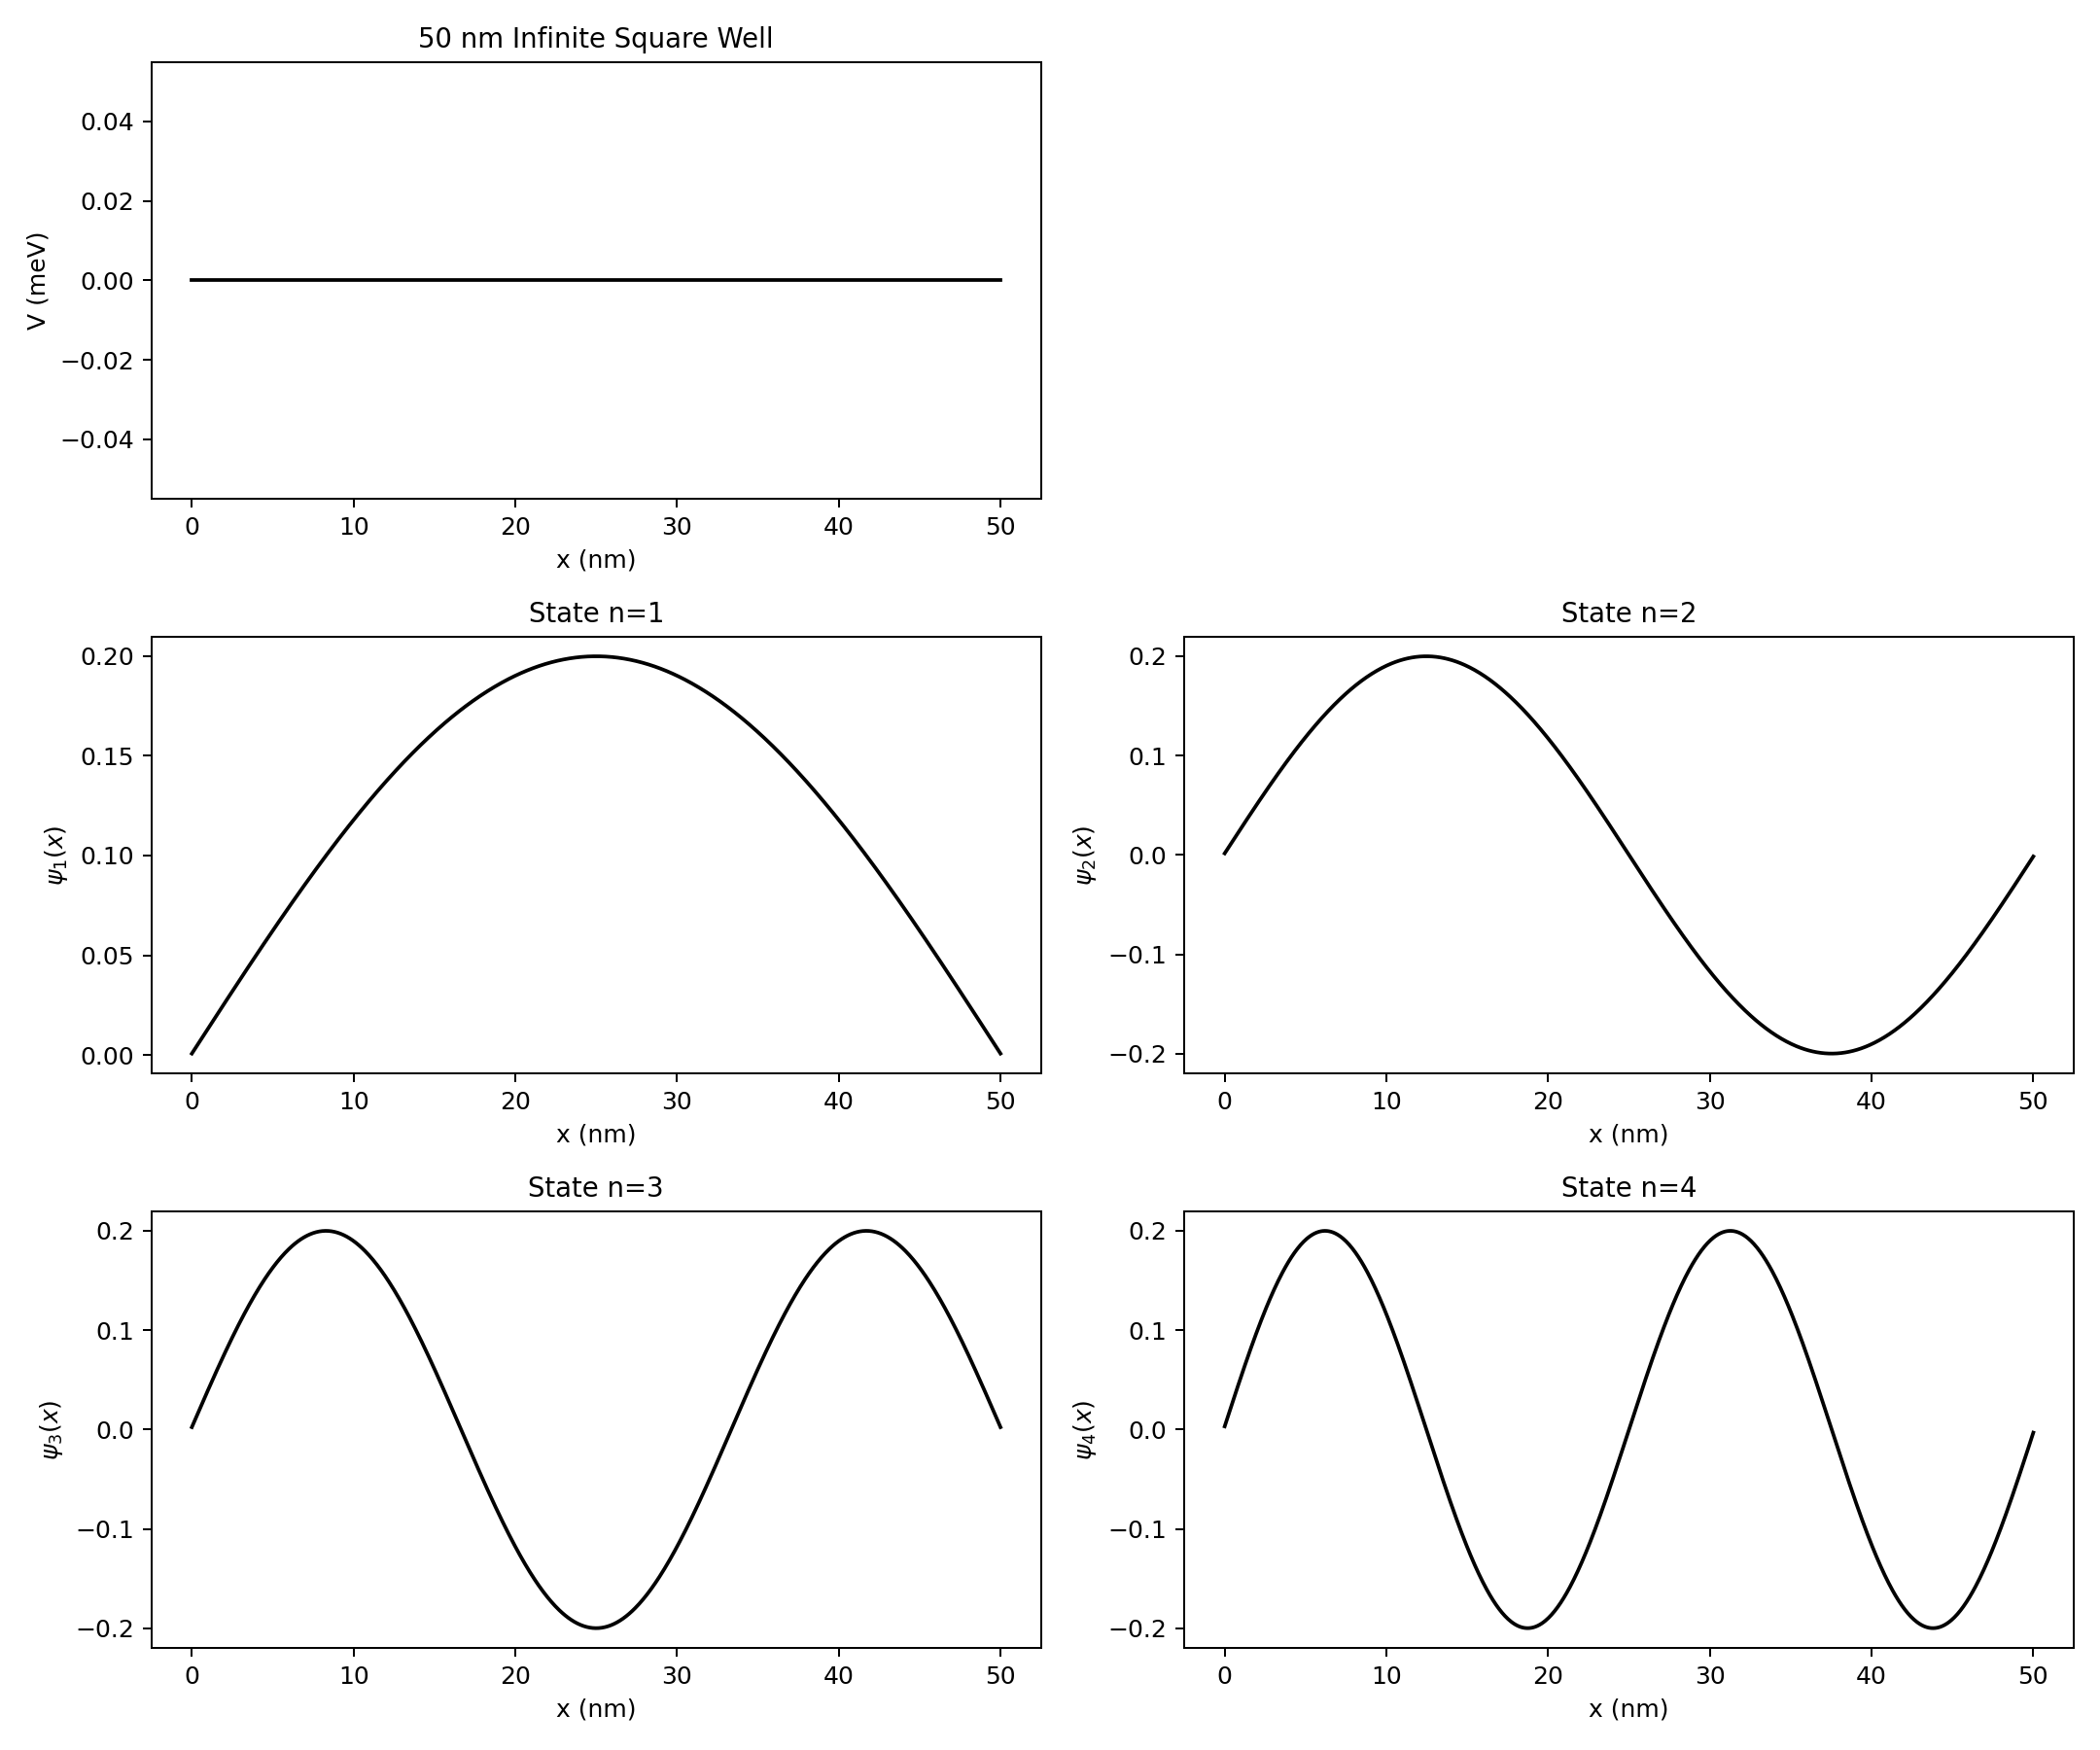
\includegraphics[width=0.82\textwidth]{outputs/infinite_well_50nm_states.png}
    \caption{50 nm 无限深势阱的势能曲线以及基态到第三激发态波函数}
\end{figure}

\section*{(b) 前10个本征能量与量子数的关系}
无限深势阱的解析公式为
\[
E_n=\frac{n^2\pi^2\hbar^2}{2mL^2}.
\]
将数值结果与解析结果比较，最大相对误差约为 $0.5115\%$，最小相对误差约为 $0.4989\%$。这说明数值结果与理论公式符合较好，偏差主要来自有限差分离散化误差。

\begin{figure}[h]
    \centering
    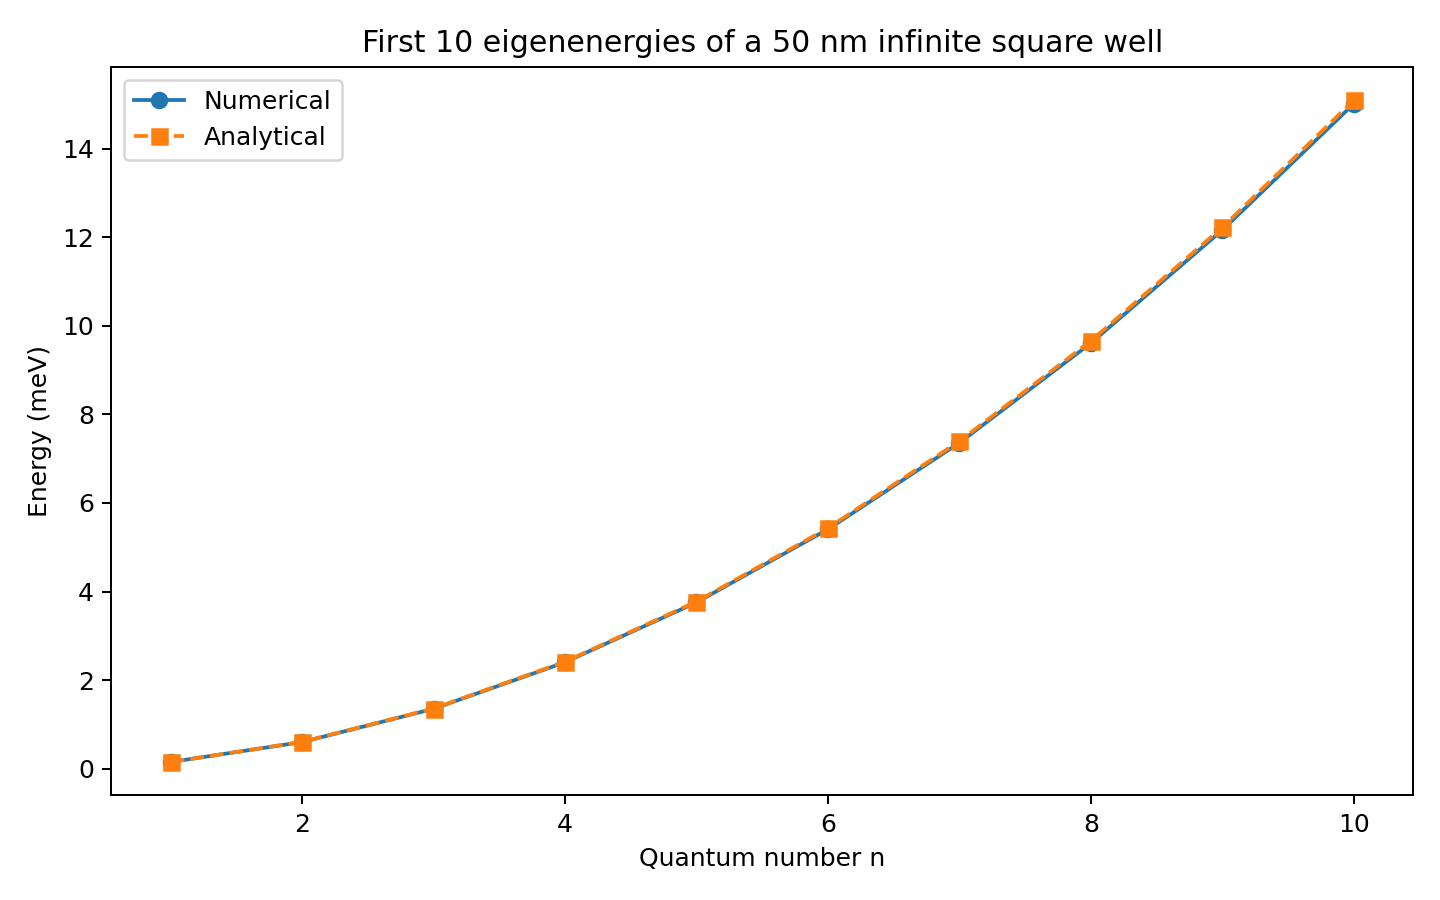
\includegraphics[width=0.65\textwidth]{outputs/infinite_well_energy_levels.png}
    \caption{50 nm 无限深势阱前10个本征能量与理论公式比较}
\end{figure}

\section*{(c) 无限深势阱宽度变化的影响}
当势阱宽度从 $10\,\mathrm{nm}$ 增大到 $100\,\mathrm{nm}$ 时，基态能量、第一激发态能量及其能量差都明显减小。数值结果例如：
\[
E_1(10\,\mathrm{nm})=3.7549\ \mathrm{meV},\quad
E_2(10\,\mathrm{nm})=15.0197\ \mathrm{meV},
\]
\[
E_1(100\,\mathrm{nm})=0.0375\ \mathrm{meV},\quad
E_2(100\,\mathrm{nm})=0.1502\ \mathrm{meV}.
\]
分析可知，势阱越宽，粒子受限越弱，动能贡献越小，因此能级整体下降，且趋势接近理论上的 $1/L^2$ 关系。

\begin{figure}[h]
    \centering
    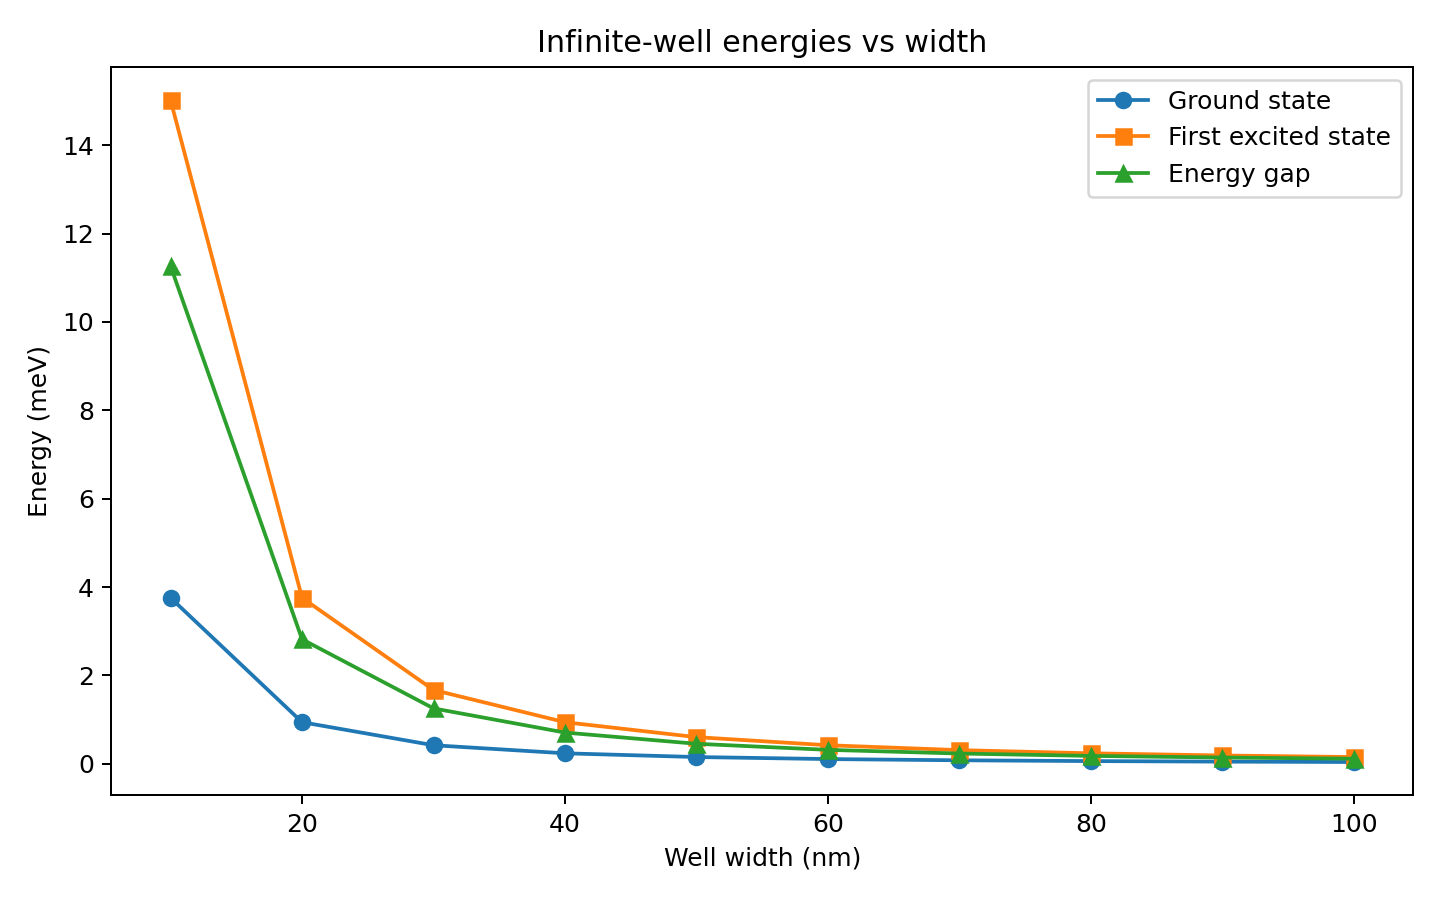
\includegraphics[width=0.7\textwidth]{outputs/infinite_well_width_scan.png}
    \caption{无限深势阱中能量与势阱宽度的关系}
\end{figure}

\section*{(d) 三角势阱的势能曲线和波函数}
对 $50\,\mathrm{nm}$ 三角势阱进行数值求解，前四个能级为
\[
18.7812,\ 43.0987,\ 59.8731,\ 75.3497\ \mathrm{meV}.
\]
与无限深势阱相比，三角势阱的波函数更集中在阱中心附近，反映出势能随位置线性增大后对粒子的额外束缚作用。

\begin{figure}[h]
    \centering
    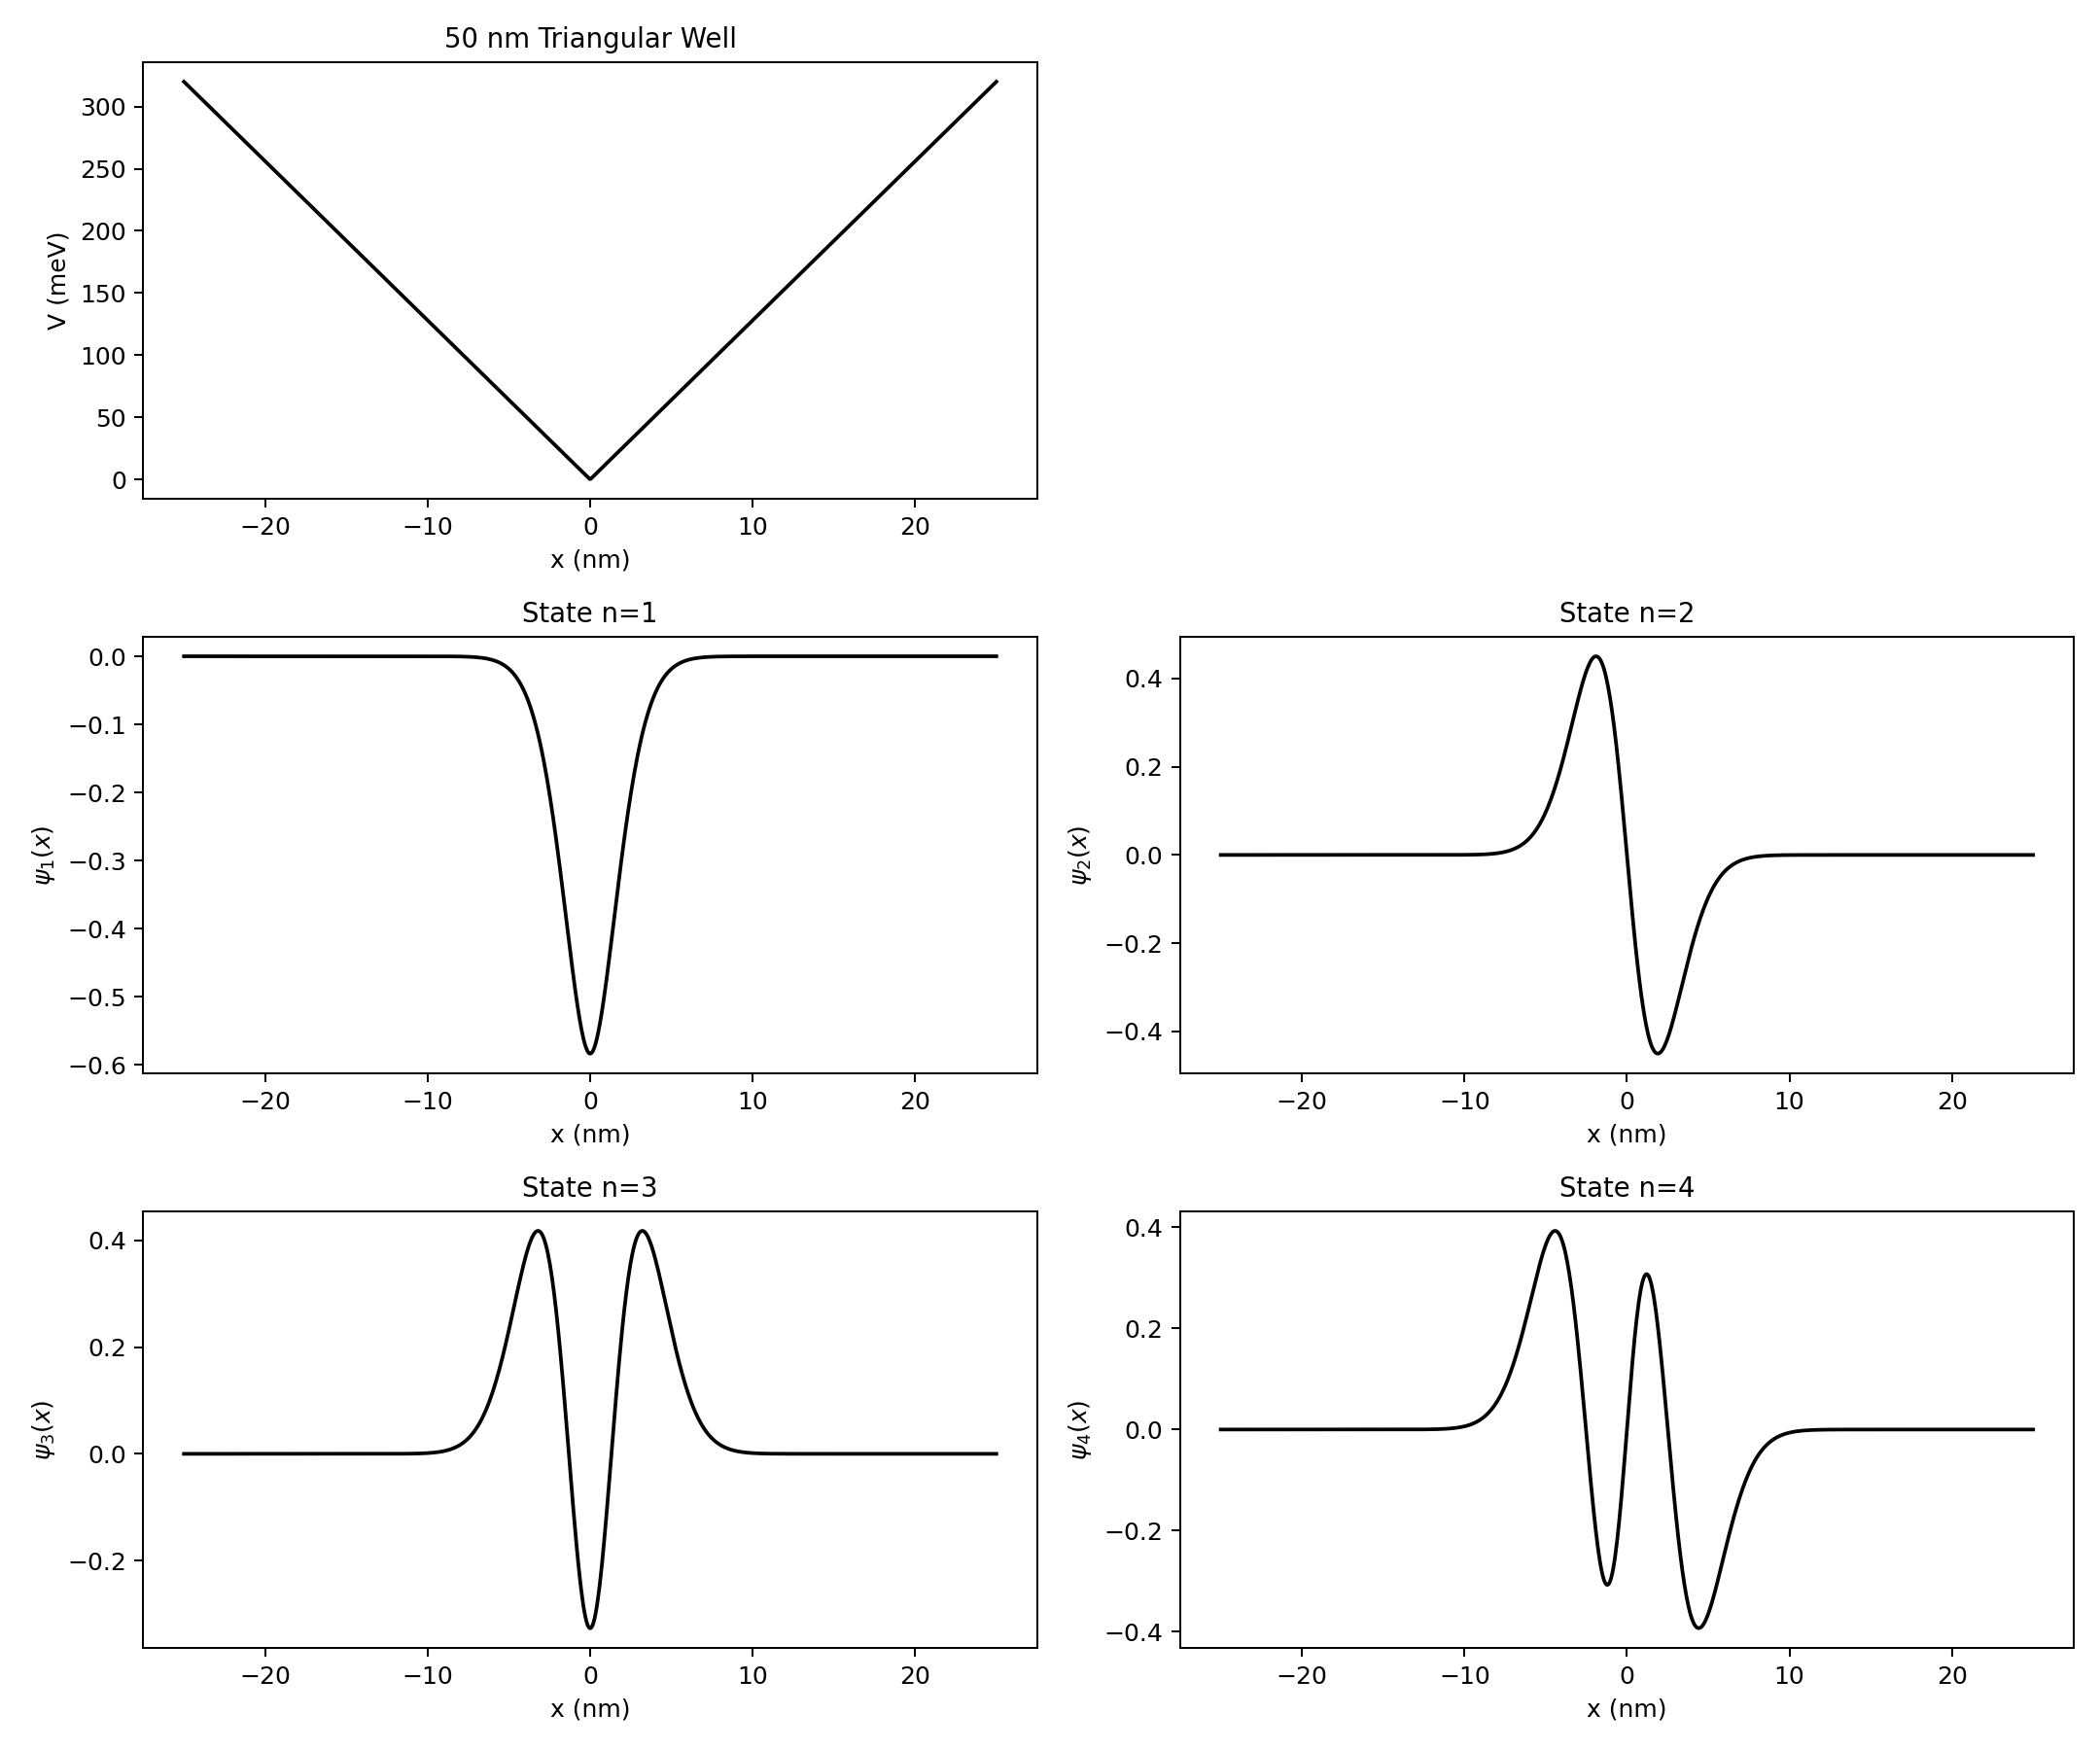
\includegraphics[width=0.82\textwidth]{outputs/triangular_well_50nm_states.png}
    \caption{50 nm 三角势阱的势能曲线以及基态到第三激发态波函数}
\end{figure}

\section*{(e) 三角势阱宽度加倍后的比较}
保持三角势阱斜率 $dV/dx$ 不变，将宽度由 $50\,\mathrm{nm}$ 扩大到 $100\,\mathrm{nm}$ 后，低能级几乎不变：
\[
E_1(50\,\mathrm{nm})=18.7812\ \mathrm{meV},\quad
E_1(100\,\mathrm{nm})=18.7820\ \mathrm{meV}.
\]
在保持横坐标区间一致后可以看到，$50\,\mathrm{nm}$ 和 $100\,\mathrm{nm}$ 的基态、第一激发态波函数几乎完全重合，因此原图中黑色曲线会被后绘制的红色曲线大部分覆盖。为更清楚地比较两者，图中将 $50\,\mathrm{nm}$ 曲线画成黑色虚线，并额外给出了差值曲线 $\psi_{100}-\psi_{50}$。从差值图可以看出，两者仅存在极小差别。

其原因是：低能态主要局域在阱中心附近，而当三角势阱斜率保持不变时，中心区域的局部势能形状几乎没有变化。虽然势阱边界被移到了更远的位置，但低能波函数在边界附近本来就已经很小，因此宽度加倍对低能定态波函数和低能级的影响都不明显。

\begin{figure}[h]
    \centering
    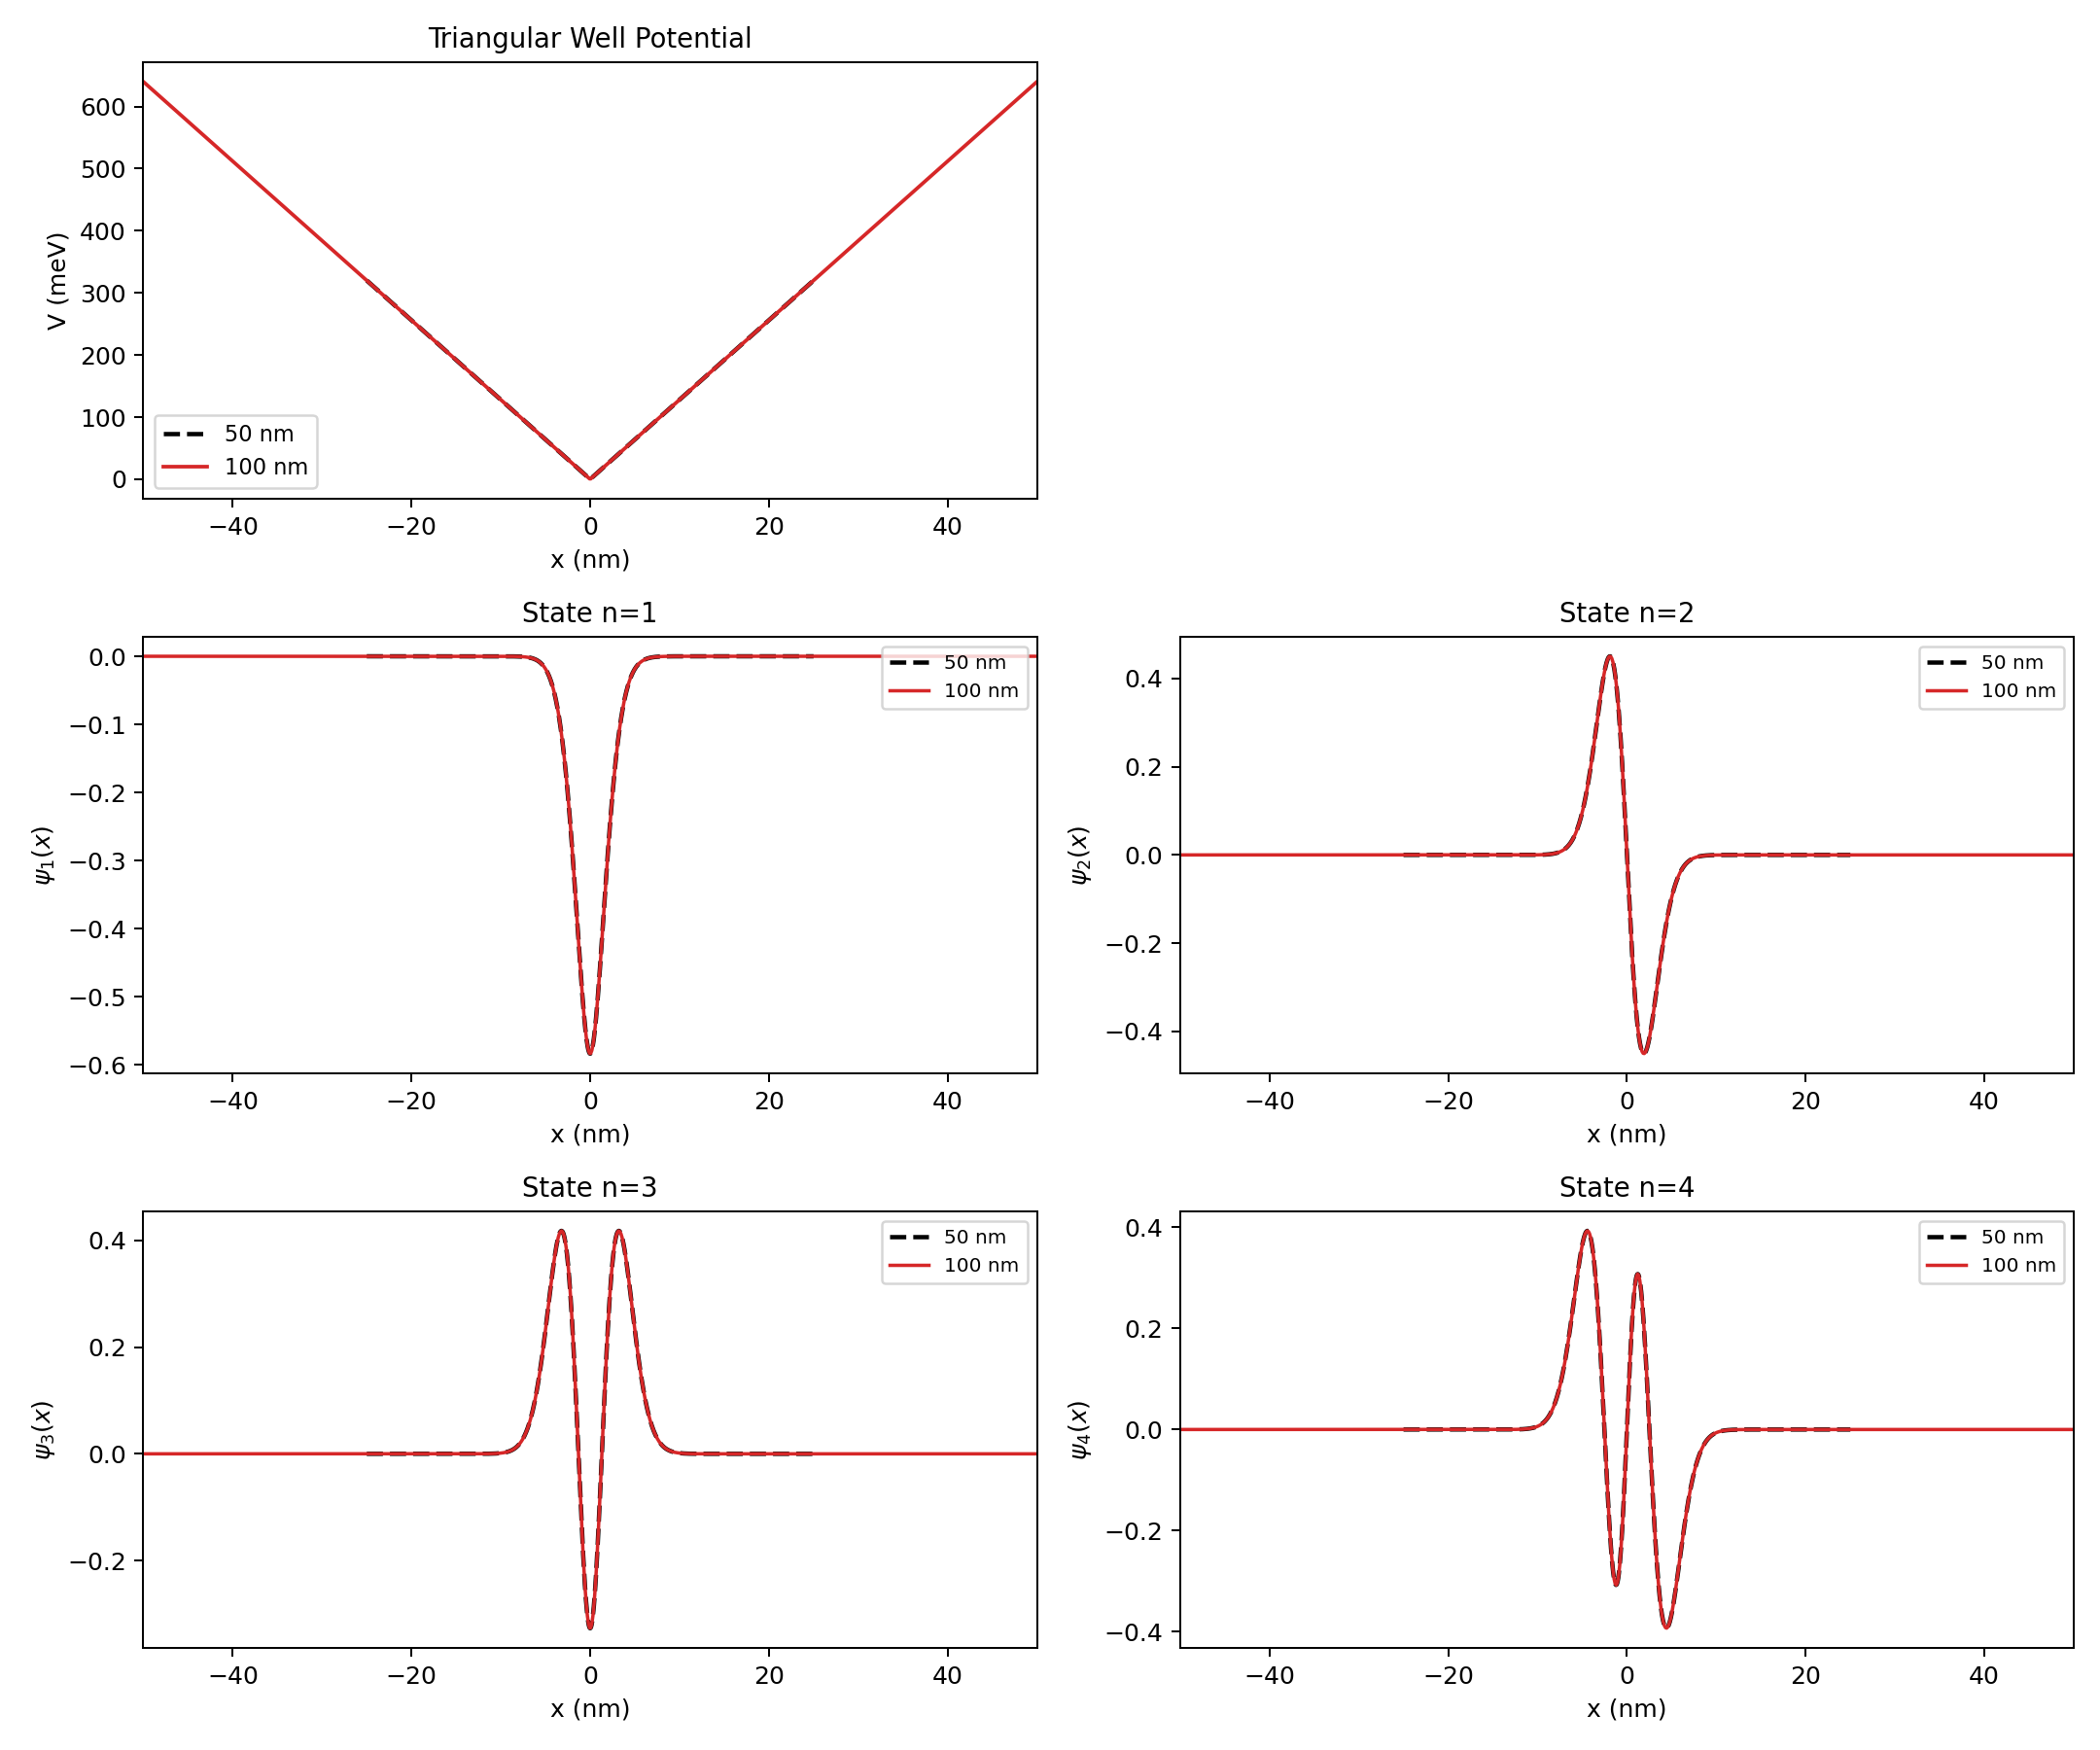
\includegraphics[width=0.82\textwidth]{outputs/triangular_well_comparison.png}
    \caption{保持斜率不变时，50 nm 与 100 nm 三角势阱的波函数、差值曲线和势能比较}
\end{figure}

\section*{(f) 抛物线势阱的结果}
题目要求抛物线经过 $(x,V)=(0,0)$、$(20\,\mathrm{nm},8\,\mathrm{eV})$ 和 $(-20\,\mathrm{nm},8\,\mathrm{eV})$ 三点，因此势函数写为
\[
V(x)=8\left(\frac{x}{20}\right)^2\ \mathrm{eV}.
\]
数值得到前四个能级为
\[
27.6505,\ 82.9454,\ 138.2277,\ 193.4974\ \mathrm{meV}.
\]
相邻能级差分别为
\[
55.2948,\ 55.2823,\ 55.2698\ \mathrm{meV}.
\]
这些能级差近似相等，说明该抛物线势阱具有典型的简谐振子特征，即相邻能级近似等间距。

\begin{figure}[h]
    \centering
    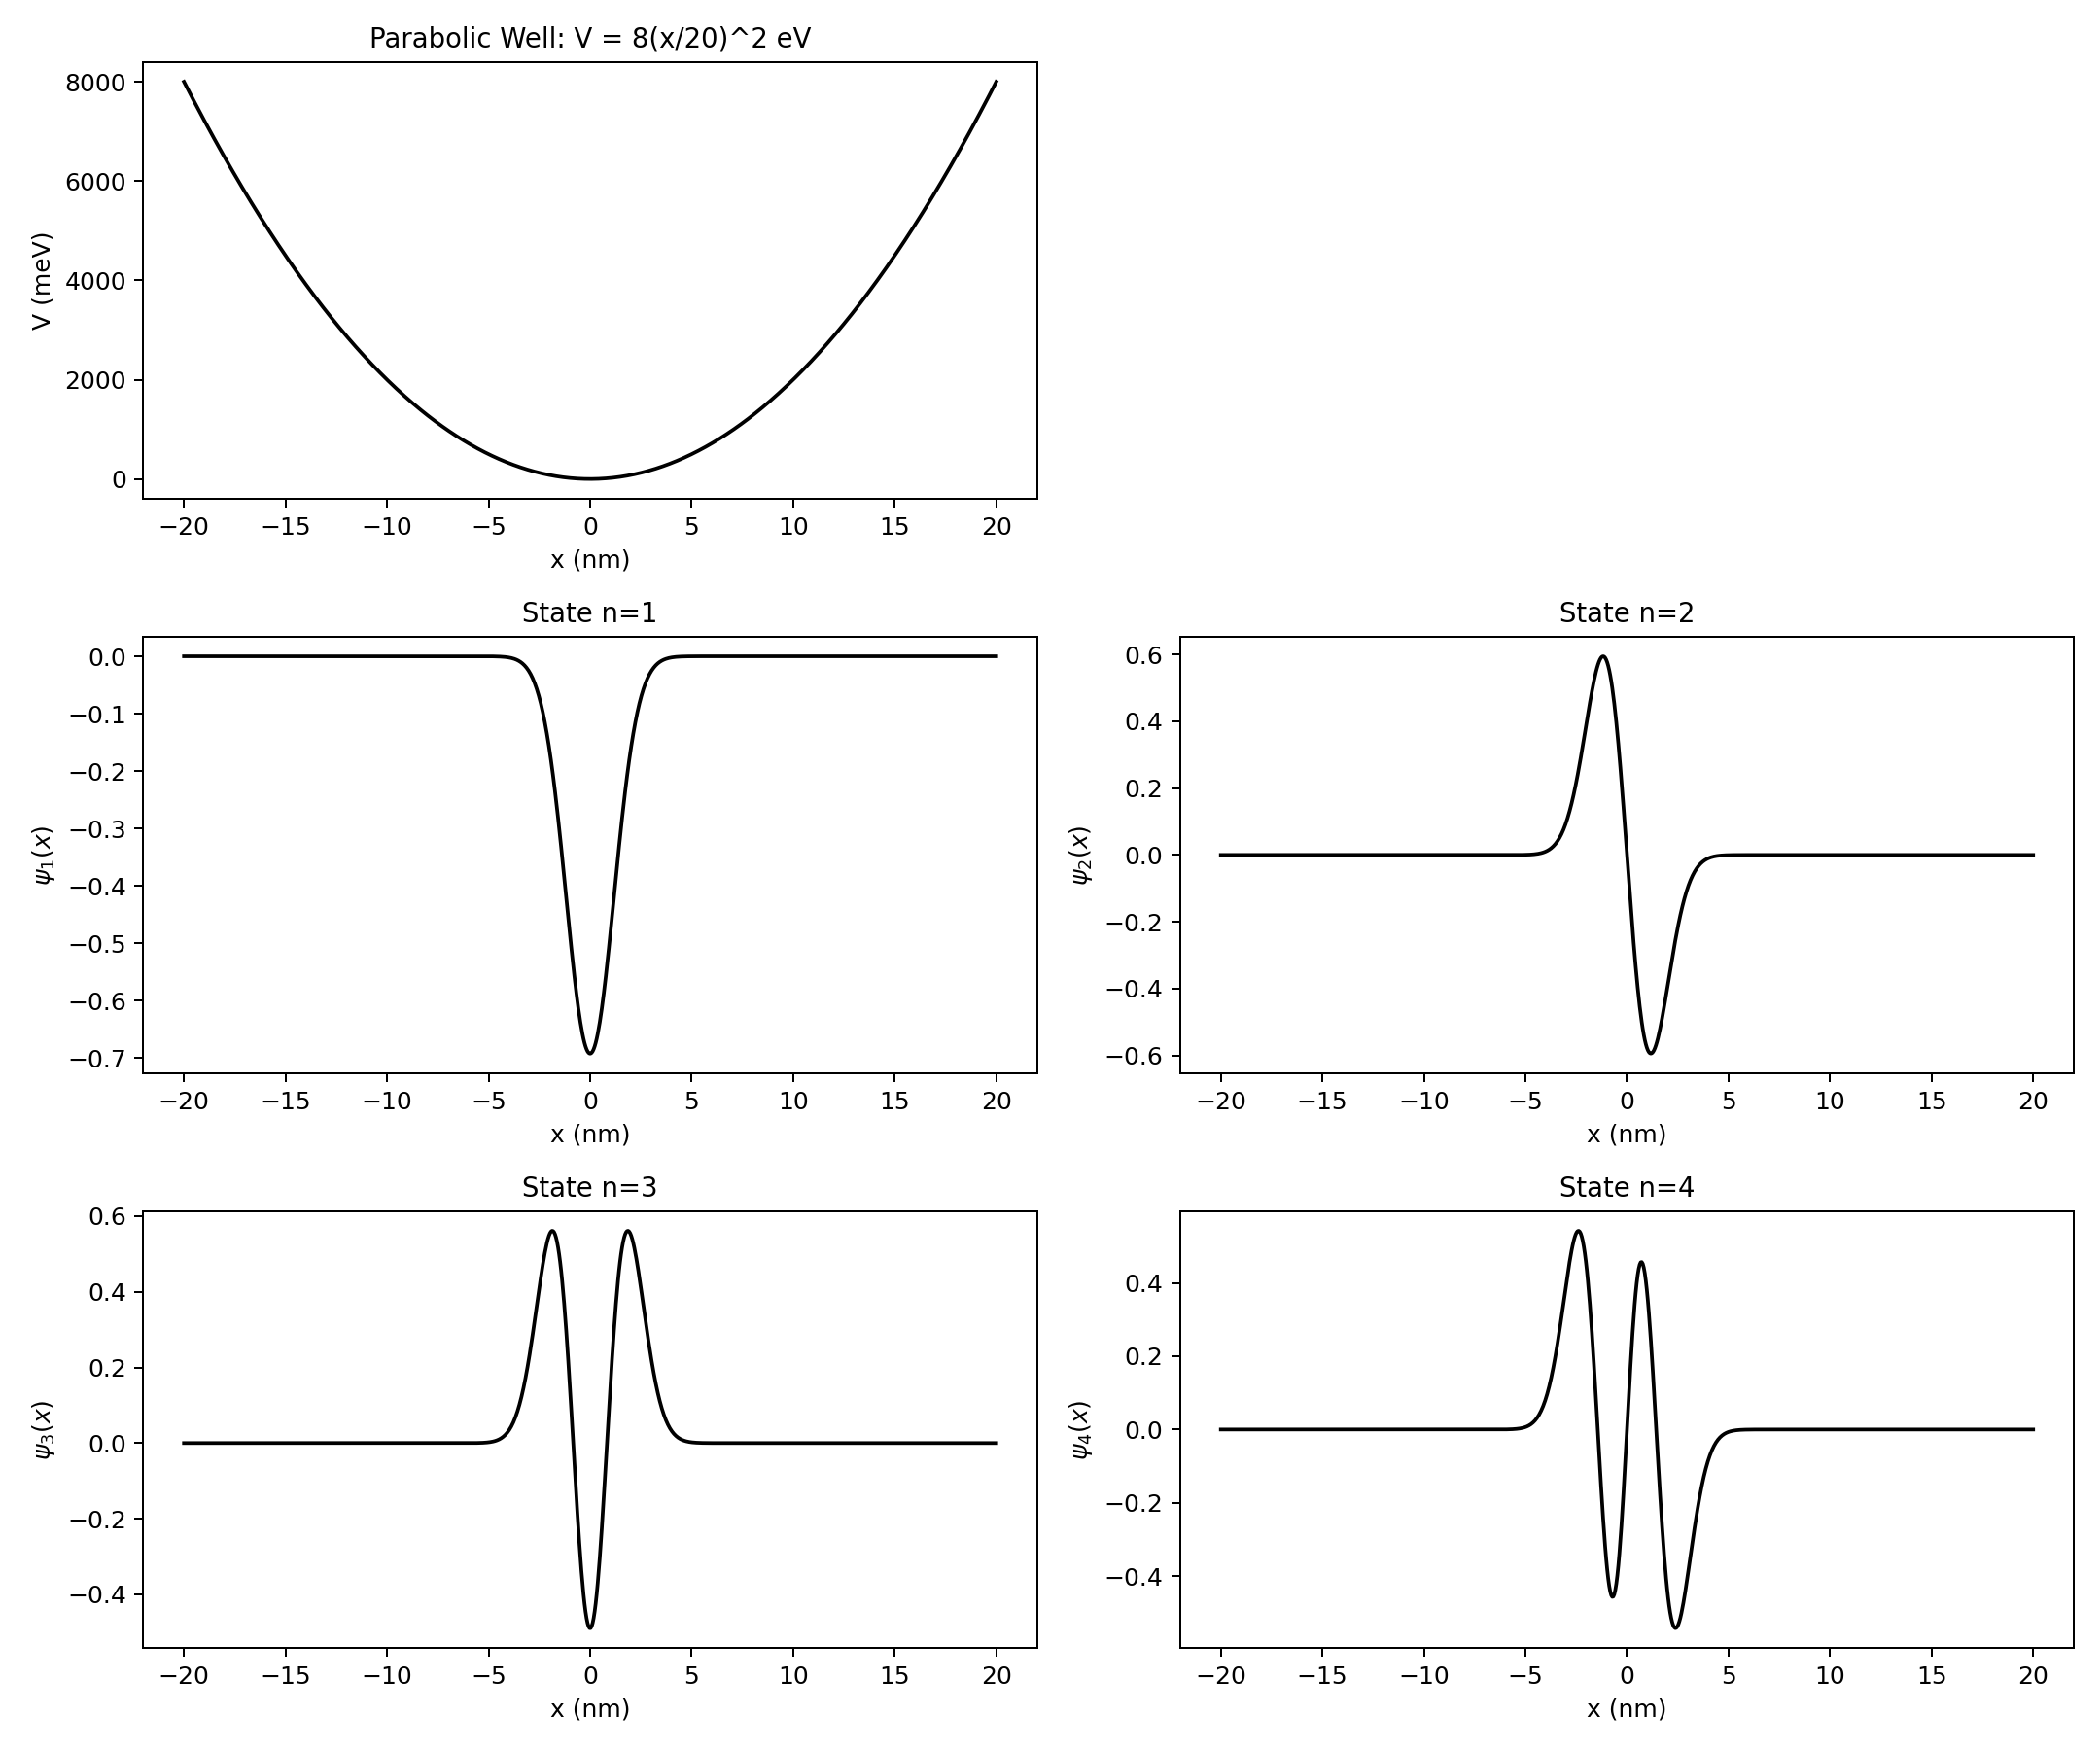
\includegraphics[width=0.82\textwidth]{outputs/parabolic_well_states.png}
    \caption{抛物线势阱的势能曲线以及基态到第三激发态波函数}
\end{figure}

\section*{总结}
本次数值计算结果与理论分析总体一致。对于无限深势阱，能级满足 $E_n\propto n^2$，且随势阱宽度增大按约 $1/L^2$ 下降；对于三角势阱，低能态主要由中心附近的局部势能决定；对于抛物线势阱，相邻能级差近似不变，体现了简谐振子型势阱的物理特征。说明有限差分方法能够有效处理不同势阱结构下的一维本征态问题。

\end{document}
